\subsubsection{\theoryC{Heavy singlet scalars at HL- and HE-LHC}}
\contributors{Dario Buttazzo, Filippo Sala, Andrea Tesi}\rt{There are comments to address.}
%{\bf Author(s): Dario Buttazzo$^{a,1}$, Filippo Sala$^{b,2}$, Andrea Tesi$^{c,3}$}\\
%
%{\it \small $^a$ INFN, sezione di Pisa, Largo Pontecorvo 3, I-56127 Pisa, Italy}\\
%{\it \small $^b$ DESY, Notkestrasse 85, D-22607 Hamburg, Germany}\\
%{\it \small $^c$ INFN, sezione di Firenze, Via G. Sansone 1, I-59100 Sesto F.no, Italy}\\
%{\small $^1$ dario.buttazzo@pi.infn.it, $^2$ filippo.sala@desy.de $^3$ andrea.tesi@fi.infn.it}\\
%Ackn: The work of F.S. is partly supported by a PIER Seed Project funding (Project ID PIF-2017-72).


%\subsubsection{Motivation}
%\paragraph*{Motivation}

The existence of extended Higgs sectors is predicted in several motivated extensions of the Standard Model.
In particular, extra Higgses that are singlets under the SM gauge group arise in some most natural BSM construction, like the next-to-minimal supersymmetric Standard Model (NMSSM, see~\cite{Ellwanger:2009dp} for a review), as well as in Twin \cite{Chacko:2005pe} and Composite~\cite{Contino:2010rs,Panico:2015jxa} Higgs models (TH and CH models).
Independently of the hierarchy problem of the Fermi scale, extra singlets constitute a minimal possibility to realise a first-order electroweak (EW) phase transition~\cite{Pietroni:1992in,Curtin:2014jma,Craig:2014lda}, which is a necessary condition to achieve EW baryogenesis.
These considerations constitute a strong case for the experimental hunt of extra singlet-like scalar particles.
It is the purpose of this Section, which updates the work of \citeref{Buttazzo:2015bka}, to review the experimental status of the searches for such scalars, and to determine the reach of the HL- and HE-LHC. To keep this contribution brief, we focus on the case where the extra singlet is heavier than the Higgs boson.

%\subsubsection{Current exclusions and future reaches}
%\paragraph*{Current exclusions and future reaches}
\label{sec:singlets_general}

\underline{Framework}. We add to the SM a real scalar field $\phi$, so that the most general renormalizable Lagrangian reads \begin{equation}
\mathcal{L} = \mathcal{L}_{\rm SM} + \frac{1}{2}(\partial S)^2  - \mu_S^2 S^2 - a_{HS} |H|^2S- \lambda_{HS} |H|^2S^2- a_S S^3 - \lambda_S S^4\,,
\end{equation}
where $H$ is the SM Higgs doublet. 
Unless a $Z_2$ symmetry is enforced ($a_{HS} = a_S = 0$), and is not spontaneously broken, the singlet mixes with the SM Higgs as
\begin{equation}
\phi = -s_\gamma\,h_0 + c_\gamma\,s_0, \qquad h = s_\gamma\,s_0 + c_\gamma\,h_0\,,
\end{equation}
where $h_0$ and $s_0$ are the neutral \cpeven degrees of freedom contained in $H$ and $S$, $h$ and $\phi$ are the resulting mass eigenstates, and $s_\gamma, c_\gamma$ are the sine and cosine of their mixing angle $\gamma$. The signal strengths $\mu$ of $h$ and $\phi$ into SM particles, defined as cross-section times branching ratio, read
%
\begin{align}
\mu_h &= c_\gamma^2 \, \mu_{\rm SM}, &
\mu_{\phi \to VV, ff} &= s_\gamma^2 \,\mu_{\rm SM} (m_\phi)\cdot (1 - {\rm BR}_{\phi \to hh}), &
\mu_{\phi \to hh} &= s_\gamma^2 \, \sigma_{\rm SM} (m_\phi)\cdot {\rm BR}_{\phi \to hh},
\end{align}
where $\sigma_{\rm SM}$ is the production cross-section of a SM Higgs boson, and $\mu_{\rm SM}$ is its signal strength into the pair of SM particles of interest.

\underline{Constraints from Higgs couplings}. The couplings of the SM-like Higgs boson $h$ to other SM particles are all reduced by the same amount $c_\gamma$, independently of $m_\phi$.
A combined ATLAS and CMS fit to Higgs coupling measurements from 8~TeV data yields the $2\sigma$ limit~\cite{Khachatryan:2016vau} $s_\gamma^2 \lesssim 0.12$, and the sensitivity reached with 36~fb$^{-1}$ of data at 13~TeV is comparable~\cite{CMS-PAS-HIG-17-031,ATLAS-CONF-2018-004}. The HL- and HE-LHC are expected to probe values of $s_\gamma^2$ at, and possibly slightly below, the 5\% level.\rt{Where does this number appear in the WG2 report? We need to refer to it here.} The current exclusion and future reach from Higgs coupling measurements is shown in \fig{fig:ModelIndep}.
Constraints on the mixing angle from EW precision tests are subdominant with respect to those from Higgs coupling measurements, see e.g.~\citeref{Carena:2018vpt}.
%
\begin{center}
\begin{figure}
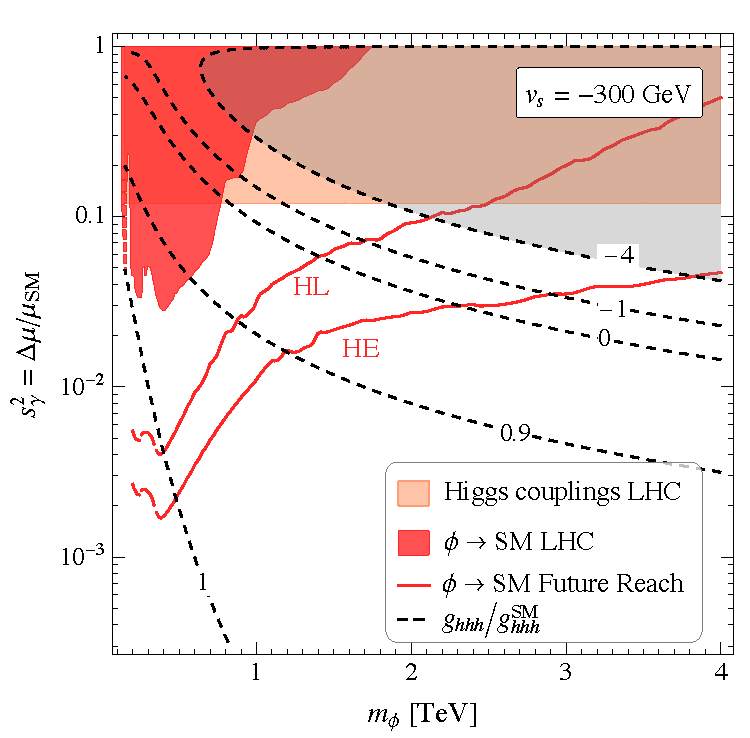
\includegraphics[width=0.49\textwidth]{\main/section7OtherSignatures/img/PlotDirectTriple_vSm300}\,
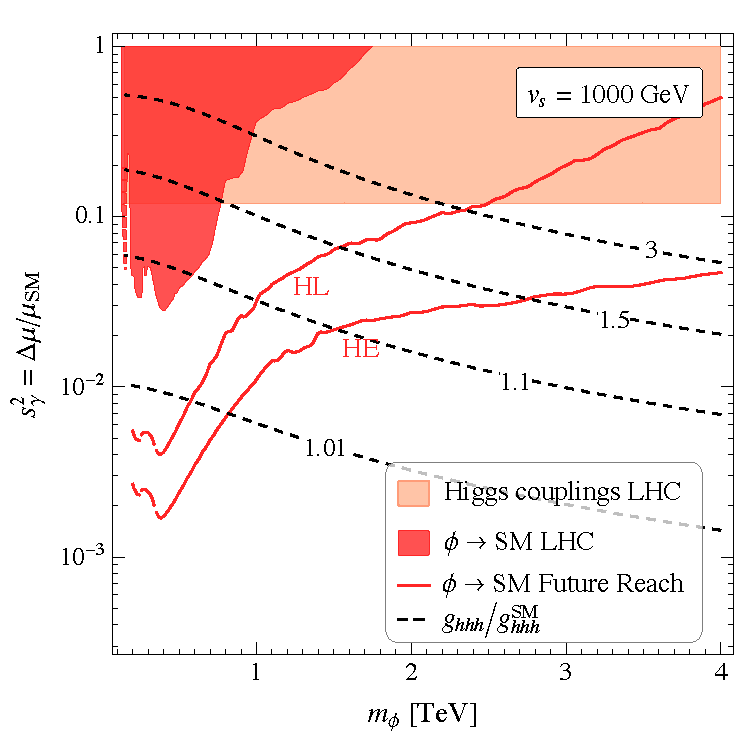
\includegraphics[width=0.49\textwidth]{\main/section7OtherSignatures/img/PlotDirectTriple_vS1000}
\caption{\label{fig:ModelIndep} Shaded: LHC exclusions from resonance searches (dark red), Higgs coupling measurements (light red) and double Higgs production (gray). Dashed black lines are contours of constant ratio between the trilinear Higgs coupling and its SM value, continuous red lines are expected sensitivities from resonance searches at the HL- and HE-LHC. The singlet \vev $v_s$ is fixed to $-300$~GeV(right) and to $1000$~GeV(left).}
\end{figure}
\end{center}

\underline{Constraints from Trilinear Higgs coupling}. The trilinear Higgs coupling $g_{hhh}$ depends on $\gamma$, $m_\phi$, and on the singlet \vev $v_s$, while its dependence on all other parameters is very mild~\cite{Buttazzo:2015bka} (we fix for definiteness $\lambda_S = \lambda_{HS} = 0.5$).
We show its ratio with respect to its SM value in \fig{fig:ModelIndep}, for two representative values of $v_s$. The gray shaded region comes from a rough bound on $g_{hhh}$ that we extract from \citeref{Aaboud:2018knk}, using the prediction of \citeref{Baglio:2012np}.\footnote{We assume that the only deviation in double Higgs production comes from deviations in $g_{hhh}$, the contribution from $pp \to \phi \to hh$ is negligibly small due to the large $m_\phi$ in the excluded region.}
Deviations of order one and larger are allowed by all current and near-future constraints, motivating in particular the HE stage of the LHC, due to the increase of the sensitivity to $g_{hhh}$ with energy. \rt{Refer again to the right part of the Higgs report.}

\underline{Constraints from direct searches of the extra singlet}.
The collider phenomenology of $\phi$ is fully controlled by only 3 parameters, $m_\phi$, $\gamma$ and ${\rm BR}_{\phi \to hh}$. Analogously to the case of the triple Higgs coupling $g_{hhh}$, ${\rm BR}_{\phi \to hh}$ depends dominantly on the model parameters $v_s$, $\gamma$, and $m_\phi$~\cite{Buttazzo:2015bka}. Moreover, because of the Goldstone boson equivalence theorem, it reaches the asymptotic value ${\rm BR}_{\phi \to hh} = {\rm BR}_{\phi \to ZZ} = 25\%$ for $m_\phi \gg m_h$, further reducing the number of parameters relevant for the phenomenology of $\phi$. %In what follows, for simplicity we fix ${\rm BR}_{\phi \to hh}$ to its asymptotic value.
Current resonance searches at the LHC exclude the red shaded area in \fig{fig:ModelIndep}, and are dominated by the CMS combined $ZZ$ search in \citeref{Sirunyan:2018qlb} at 13 TeV with 36~fb$^{-1}$ of data. We rescale the expected sensitivity at 13 TeV~\cite{Sirunyan:2018qlb} at higher energies and luminosities using quark parton luminosities, with a procedure analogous to the one presented in \citeref{Buttazzo:2015bka}. Our results for the expected sensitivities at the HL (14 TeV, 3~ab$^{-1}$) and HE (27 TeV, 3~ab$^{-1}$) stages of the LHC are also shown in \fig{fig:ModelIndep}.
Direct searches for the new scalar constitute the strongest probe of the parameter space of these models for $m_\phi$ below about a TeV, while larger masses are (and will be) probed more efficiently by deviations in Higgs couplings, thus making these two strategies complementary in the exploration of these  models.

%\subsubsection{Interpretation in the NMSSM and in Twin and Composite Higgs}
%\paragraph*{Interpretation in the NMSSM and in Twin and Composite Higgs}
%
\begin{center}
\begin{figure}
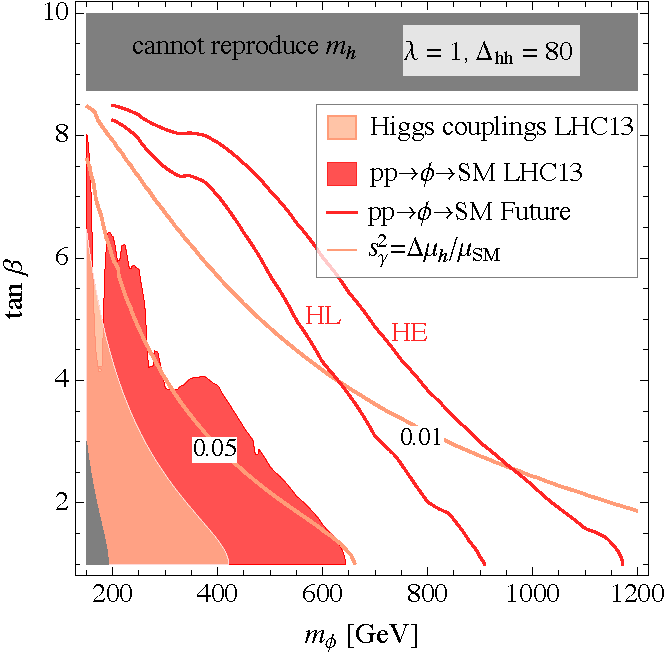
\includegraphics[width=0.47\textwidth]{\main/section7OtherSignatures/img/NMSSM_HEHL_l1_Delta80} \;
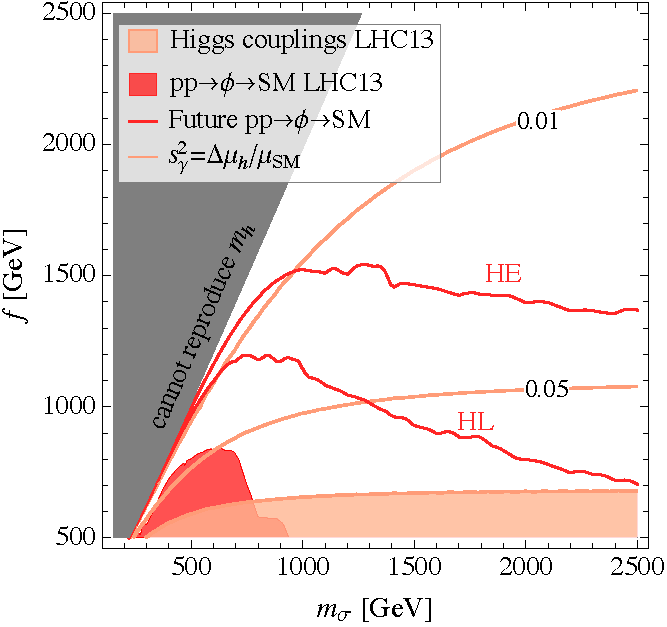
\includegraphics[width=0.50\textwidth]{\main/section7OtherSignatures/img/TH_HEHL_NoInv}
\caption{\label{fig:NMSSM_TH}
Shaded: LHC exclusions from resonance searches (dark red) and Higgs coupling measurements (light red). %Dark gray shaded areas are unphysical.
Left: NMSSM with couplings $\lambda = 1$ and with $\Delta_{hh} = 80$~GeV. Right: Twin and Composite Higgs models. %, where in the shaded area in the bottom-right corner one has $\Gamma_\sigma > m_\sigma$.
See text for more details.
}
\end{figure}
\end{center}
%

\underline{Implications for the NMSSM}. The NMSSM adds to the MSSM particle content a singlet $S$, so that the superpotential reads $W = W_{\rm \tiny MSSM} + \lambda\,S H_u H_d + f(S)$.
The fine-tuning needed to reproduce the EW scale is parametrically alleviated, with respect to the MSSM, and for a given value of the stop and gluino masses, by a factor $\lambda/g$, see e.g.~\citerefs{Barbieri:2006bg,Hall:2011aa,Agashe:2012zq,Gherghetta:2012gb}.
Naturalness arguments thus favour a large $\lambda$, that is however bounded from above by perturbativity.
Assuming the masses of the extra Higgs bosons in the TeV range, a model with $\lambda \simeq 2$ becomes strongly coupled at scales of order 10 TeV, and to have a perturbative coupling up to the GUT scale one needs $\lambda \lesssim 0.7$~\cite{Espinosa:1991gr}.\footnote{It is conceivable that a strong sector exists at the scale where $\lambda$ becomes non-perturbative, and without affecting the success of GUT in the NMSSM, see e.g. the model in \citeref{Barbieri:2013hxa} and references therein.}

Here we employ the economical parametrization of the NMSSM scalar sector put forward in \citerefs{Barbieri:2013hxa,Barbieri:2013nka}.
We then assume the extra Higgs doublet to be (slightly) decoupled, and we study the phenomenology of the Higgs-singlet scalar sector, which can be described by 4 free parameters
\begin{equation}
m_\phi, \quad \lambda,\quad t_\beta, \quad \Delta_{hh},
\label{eq:singlets_NMSSMpars}
\end{equation}
where $t_\beta$ is the ratio of the up and down Higgs \vevs, and $\Delta_{hh}$ encodes the radiative contribution to the SM-like Higgs mass $m_h^2 \lesssim m_Z^2 \,c^2_{2\beta} + \lambda^2 \,v^2\,s^2_{2\beta}/2 + \Delta_{hh}^2$. %, $\Delta_{hh} \simeq $.
The phenomenology discussed in the previous section is displayed, for the NMSSM, in the left-hand panel of \fig{fig:NMSSM_TH}.
We have fixed $\Delta_{hh} = 80$~GeV, a value obtainable for stop masses and mixing in the range of 1-2 TeV.
The precise value of $\Delta_{hh}$ does not affect the Higgs sector phenomenology as long as it is within order 10\% of 80 GeV. We have also fixed $\lambda =1$, smaller values would make all the exclusions and sensitivities weaker, while larger values would make them stronger.

As seen in \fig{fig:NMSSM_TH} left, direct searches for the extra singlet are expected to constitute the most promising probe of the $\phi - h$ parameter space. %, the reason being the fast decrease of the mixing angle $\gamma$ with increasing $m_\phi$ in the NMSSM.
Higgs coupling measurements will give a reach at most comparable to the one of resonance searches, and they will constitute a crucial complementary access to the parameter space of NMSSM scalars. Deviations in the trilinear Higgs coupling depend on more parameters than those in \eq{eq:singlets_NMSSMpars}, and can reach around 50\% or more if $\lambda \gtrsim 1$, see \citeref{Sala:2015lza} for a precise quantification.

\underline{Twin and Composite Higgs}.
In both TH and CH models, the SM-like Higgs boson is the pseudo-Goldstone boson associated to the spontaneous breaking of a global symmetry at a scale $f$. The EW fine-tuning of CH models is comparable to the one of typical SUSY constructions, while TH models can achieve a tuning as good as the irreducible factor $v^2/f^2$ (mainly because the top partners are neutral under color, and can thus be light).
The radial scalar mode $\sigma$ associated to the pseudo-Goldstone Higgs has a mass $m_\sigma \sim g_* f$, where the size of $g_*$ corresponds to the typical one of the coupling of the UV completion.
TH models with weakly coupled UV completions
feature an extra scalar singlet that can be light, see e.g. \citerefs{Katz:2016wtw,Badziak:2017syq}.
The hunt for the extra scalar is a crucial test of TH models, because of the small couplings to the SM of the rest of the ``Twin'' states.

The scalar potential of TH and CH models has less free parameters, so that all the quantities relevant for the scalar phenomenology (including $g_{hhh}$ and ${\rm BR}_{\phi \to hh}$) are a function of two free parameters only, that we choose to be $f$ and $m_\sigma$.
One for example obtains $s_\gamma \approx v/f$ and  $g_{hhh} \approx 1$ up to terms suppressed by the small ratio $v^2/f^2$.
In TH, an extra freedom is given by the decay channels of $\phi$ into the Twin sector, whose branching ratio in the limit $m_\sigma \gg g f$ is fixed, through the Goldstone boson equivalence theorem, by the symmetries of the model (3/7 in the cases of $SO(8)/SO(7) \simeq SU(4)/SU(3)$). For simplicity, and because such decay is absent in CH models, we do not include it in our study.

The constraints and sensitivities discussed 
%in Section~\ref{sec:singlets_general} 
above
are displayed in the right-hand panel of \fig{fig:NMSSM_TH}.
Given our considerations above, in the case where these models are not too strongly coupled (we checked that $\Gamma_\sigma < m_\sigma$ in the whole parameter space that we show \rt{Very mild requirement. Is it also below 10-30\% of the mass or not?}), they are expected to manifest themselves first via new diboson resonances. On the contrary, their strong-coupling regime is expected to show up first in deviations in the Higgs couplings.




